% Paleta pastel alternativa
\definecolor{FixationColor}{HTML}{BFD8B8}
\definecolor{MotorColor}{HTML}{F6C28B}
\definecolor{RestColor}{HTML}{A7C5EB}
\definecolor{InterColor}{HTML}{EDE6F2}
\definecolor{CueColor}{HTML}{B5EAEA}

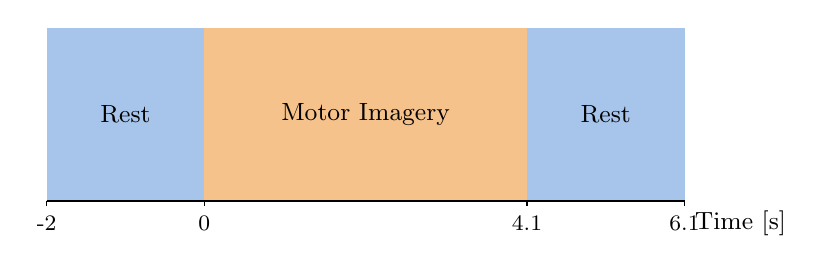
\begin{tikzpicture}
  % ===== Parámetros =====
  \def\boxheight{2.2}

  % Tiempos (s)
  \def\startRest{-2}
  \def\endRestA{0}
  \def\endMI{4.1}
  \def\endRestB{6.1}

  % ===== Bloques (SIN MARCOS) =====
  \fill[RestColor]  (\startRest,0) rectangle (\endRestA,\boxheight);
  \fill[MotorColor] (\endRestA,0)  rectangle (\endMI,\boxheight);
  \fill[RestColor]  (\endMI,0)     rectangle (\endRestB,\boxheight);

  % ===== Etiquetas internas =====
  \node[font=\small] at ({(\startRest+\endRestA)/2},{0.5*\boxheight}) {Rest};
  \node[font=\small] at ({(\endRestA+\endMI)/2},{0.5*\boxheight}) {Motor Imagery};
  \node[font=\small] at ({(\endMI+\endRestB)/2},{0.5*\boxheight}) {Rest};

  % ===== Eje X =====
  \draw[thick] (\startRest,0) -- (\endRestB,0)
        node[below right,font=\small] {Time [s]};

  \foreach \x/\lbl in {
      \startRest/-2,
      \endRestA/0,
      \endMI/4.1,
      \endRestB/6.1}{
    \draw (\x,0) -- ++(0,-2pt) node[below,font=\footnotesize] {\lbl};
  }

\end{tikzpicture}
